{\actuality} На протяжении десятилетий в качестве мотивации для многих исследований в области звездной астрономии авторы публикаций приводят фразу: <<изучение строения и формирования Галактики и ее подсистем>>. Несмотря на длительную историю, эта фраза не превратилась в пустое клише, что подтверждается перечнем научных целей космической мисси Gaia, которая уже совершила настоящий прорыв в качестве и объеме данных о разных звездных и субзвездных популяциях Млечного пути. Данная работа тоже направлена на решение указанной фундаментальной задачи. Объектами нашего внимания стали маломассивные карлики, входящие в состав галактического диска и гало. Мы фокусируемся на добыче и интерпретации информации о количестве и качестве двойных и кратных систем, компоненты которых относятся к упомянутым типам звезд.

\ifsynopsis
\else
Когда употребляется словосочетание <<изучение звездной популяции>>, то понимается в первую очередь набор формальных характеристик: число объектов, пространственное распределение, кинематические свойства, диапазоны физических параметров. Для получения истинных значений всех перечисленных величин важно стремиться к полноте выборки объектов популяции. Хорошо известно, что это условие непросто соблюсти с помощью даже современных возможностей наблюдательной астрономии просто потому, что при громадных расстояниях и недостаточной светимости исследуемые звезды либо ненаблюдаемы вовсе, либо их излучение регистрируется на пределе технических возможностей. По этой причине нередко ограничиваются изучением области Галактики, которая доступна для исследований. Поэтому довольно часто рассматривается так называемая солнечная окрестность. Стоит уточнить, что в различных исследованиях радиус ближайшего окружения  Солнца варьируется от 10 до 100 пк, но зачастую даже в одном проекте размер анализируемой области Галактики на разных этапах может расти или уменьшаться в зависимости от поставленных задач.
\fi

Поскольку наше исследование посвящено звездам со светимостями от $10^{-4}$ до $10^{-2}$ от солнечной, то вполне естественно, что будут рассматриваться объекты, заключенные в гелиоцентрической сфере радиусом в 50 пк. То есть речь идет о ближайшем галактическом окружении Солнца, где можно уверенно наблюдать карликовые звезды и надеяться на полноту выборки. При обычных для звезд диска скоростях движения относительно Солнца из-за малого гелиоцентрического расстояния карлики солнечной окрестности обладают весьма значительными величинами собственных движений ( $\mu$ > 0.1~$''$/yr). До появления второго релиза миссии Gaia (и массовых определений тригонометрических параллаксов) такой анализ величин собственных движений был чуть ли не единственным способом быстрого выявления близких к Солнцу карликов. Неслучайно чаще других для отбора объектов низкой светимости привлекали каталог быстрых звезд LSPM \cite{2005AJ....129.1483L}. 
 
Интерес астрономического сообщества к маломассивной фракции звездного населения солнечной окрестности обусловлен тем, что детальное изучение кинематики и статистических свойств звездного ансамбля в этой области Галактики позволяет получить представление о генезисе околосолнечной области, тестировать модели строения и эволюции Галактики. Это отражено в целом комплексе работ (см., например, \cite{2015A&A...576A.113Z}; \cite{2015MNRAS.449.3479S}).

Как показывают результаты наблюдений космической миссии Gaia, абсолютное большинство звездного населения околосолнечной области составляют различные типы карликов (см. рисунок~\ref{fig:typ}). Проблему нехватки наблюдений и статистических данных о звездах низкой светимости, а также важность уточнения по этим данным 
эмпирических соотношений между параметрами звезд выделяют во многих работах. В частности, большой научный интерес в отношении карликов представляют уточнения зависимостей <<масса -- светимость>> \cite{2016AJ....152..141B}, <<масса -- радиус>> \cite{2014MNRAS.437.2831Z} и построение в согласии с этими зависимостями физических моделей маломассивных звёзд \cite{2013AN....334....4T}, \cite{2013ApJ...776...87S}. Отмечается, что в отличие от звезд солнечных и более масс, для которых существующие теории строения находят соответствие с наблюдениями, аналогичные модели для маломассивных объектов являются гораздо менее совершенными (см., например, \cite{2013ApJ...776...87S}). Уже упомянутые эмпирические закономерности могут служить тестами моделей строения звезд и их атмосфер, и для них важны точные астрометрические и фотометрические исследования, разносторонний подход к накоплению данных. 

\begin{figure}[pt]
  \centering
  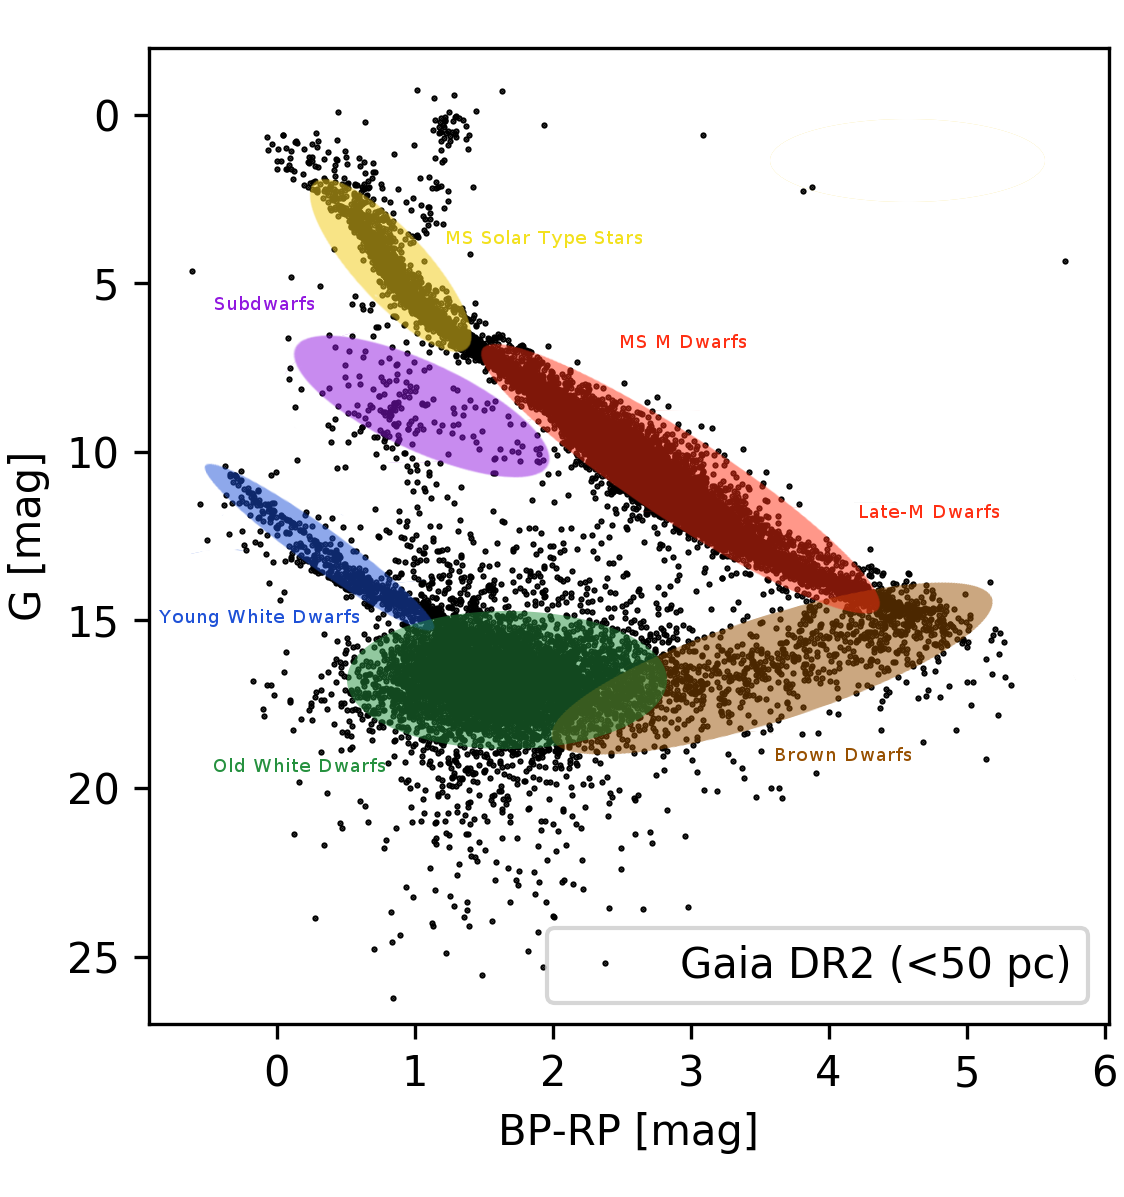
\includegraphics [scale=1.5] {gaia50types}
  \caption{На диаграмме <<показатель цвета $BP-RP$ -- абсолютная звездная величина в полосе G>> представлены звезды Gaia DR2 из ближайших окрестностей (до 50 пк). Цветными областями обозначено приблизительное разбиение звезд на группы, исходя из значений их показателей цвета и абсолютных звездных величин.}
  \label{fig:typ}
\end{figure}

\begin{figure}[pt]
  \centering
  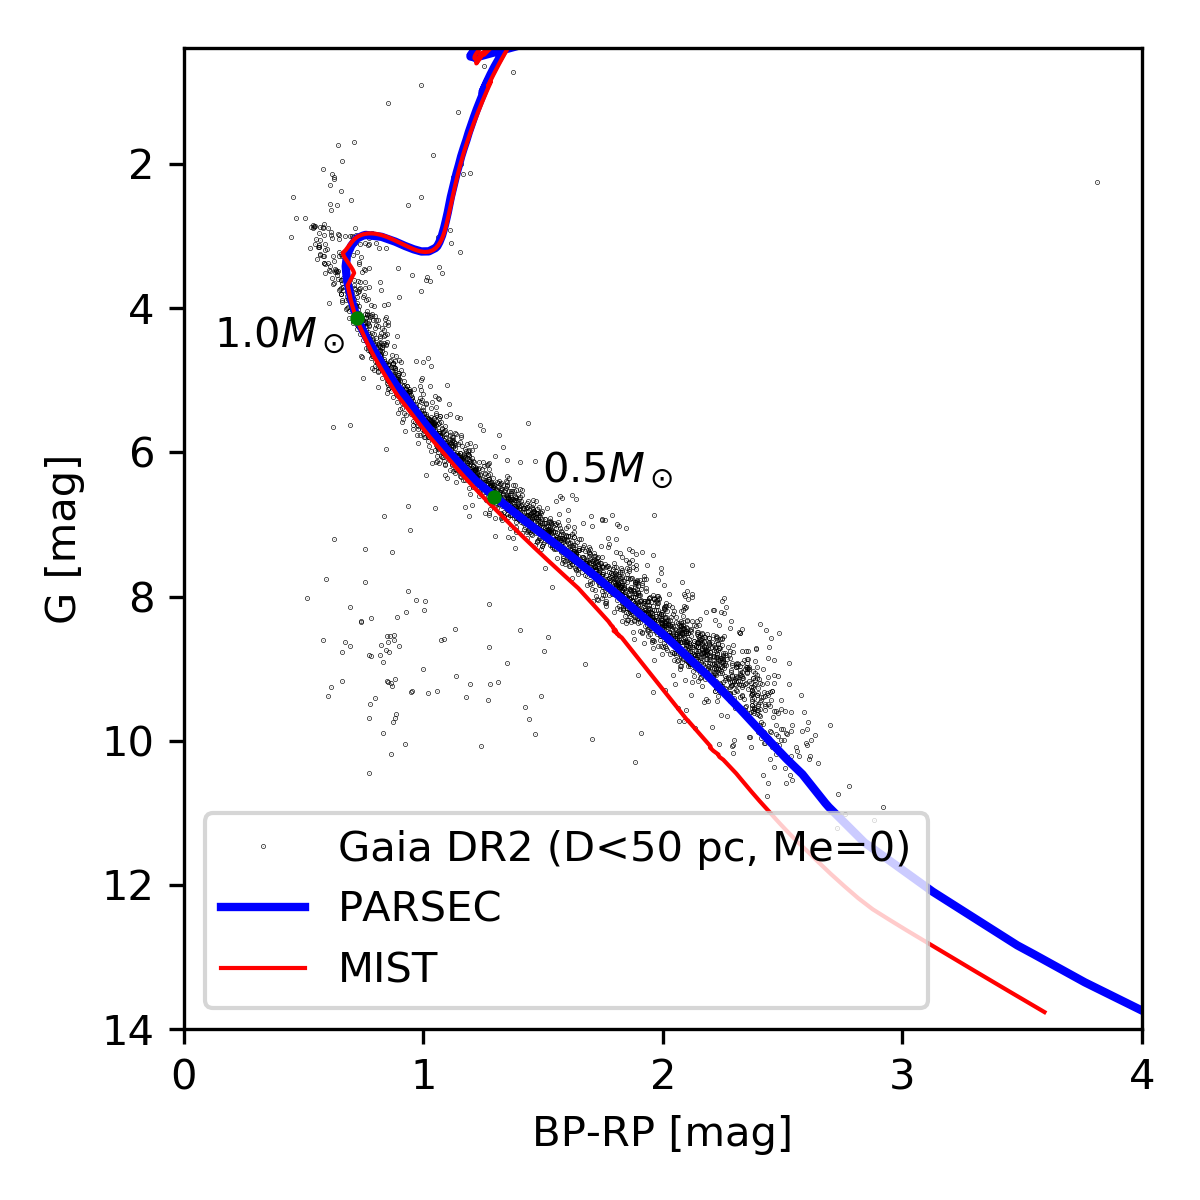
\includegraphics [scale=1.5] {parsec-mist-gaia}
  \caption{На диаграмме <<показатель цвета $BP-RP$ -- абсолютная звездная величина в полосе G>> представлены звезды Gaia DR2 из ближайших окрестностей (до 50 пк) с солнечной металличностью, соответствующие модельные изохроны проектов PARSEC и MIST, а также положения соответствующих звезд с массами 1 \(\textup{M}_\odot\) и 0.5 \(\textup{M}_\odot\).}
  \label{fig:iso}
\end{figure}

В настоящее время существует ряд проектов, нацеленных на конструирование моделей звезд различных типов. На рисунке~\ref{fig:iso} представлено сравнение звезд солнечной металличности из ближайших 50 пк по данным Gaia DR2 c модельными изохронами, построенными с помощью систем MIST \cite{2016ApJ...823..102C} и PARSEC \cite{2012MNRAS.427..127B}. Как видно из рисунка, для масс от 1 до 0.5 \(\textup{M}_\odot\) наблюдаемые данные очень хорошо согласуются с обеими изохронами, при массах менее 0.5 \(\textup{M}_\odot\) расхождение между системами изохрон весьма значительно, причем наилучшее согласие с наблюдениями имеет кривая, построенная с помощью PARSEC. Это можно объяснить в большей степени эмпирическим характером построения той части модели, которая описывает менее массивные звезды. Авторы PARSEC отмечают, что такой подход прежде всего связан с трудностью моделирования звездных атмосфер у объектов с сильным влиянием конвекционных процессов. Чтобы справиться с проблемой моделирования объектов легче $0.5 M_\odot$, авторы PARSEC вносили поправки на основе данных для пары сотен наблюдаемых затменно-двойных звезд, для которых есть хорошие кривые лучевых скоростей (см. рисунок~\ref{fig:mrr}). Но оказалось, что наблюдаемые затменно-двойные звезды слишком тесные, и соотношение масса-радиус для таких звезд не отвечает моделям одиночных звезд. Одно из предположений заключается в том, что в таких системах происходит инфляция радиуса за счёт взаимного нагрева компонент. Однако, попытка оценить такое влияние показала увеличение радиуса не более, чем на 6\,\%  при превосходстве светимости <<влияющего>> компаньона более, чем в 500 раз (см. рисунок~\ref{fig:inf}). Но эта работа продемонстрировала сложность физики взаимодействий в тесной системе маломассивных карликов, где имеют место  взаимные приливные деформации компонент. Поэтому крайне интересны двойные системы, состоящие из маломассивных звезд и при этом достаточно удаленные друг от друга, чтобы зависимость <<масса -- радиус>> соответствовала одиночным звездам. Собственно поиск таких систем и есть одна из целей настоящего исследования.

\begin{figure}[pt]
  \begin{minipage}[ht]{1\linewidth}\centering
    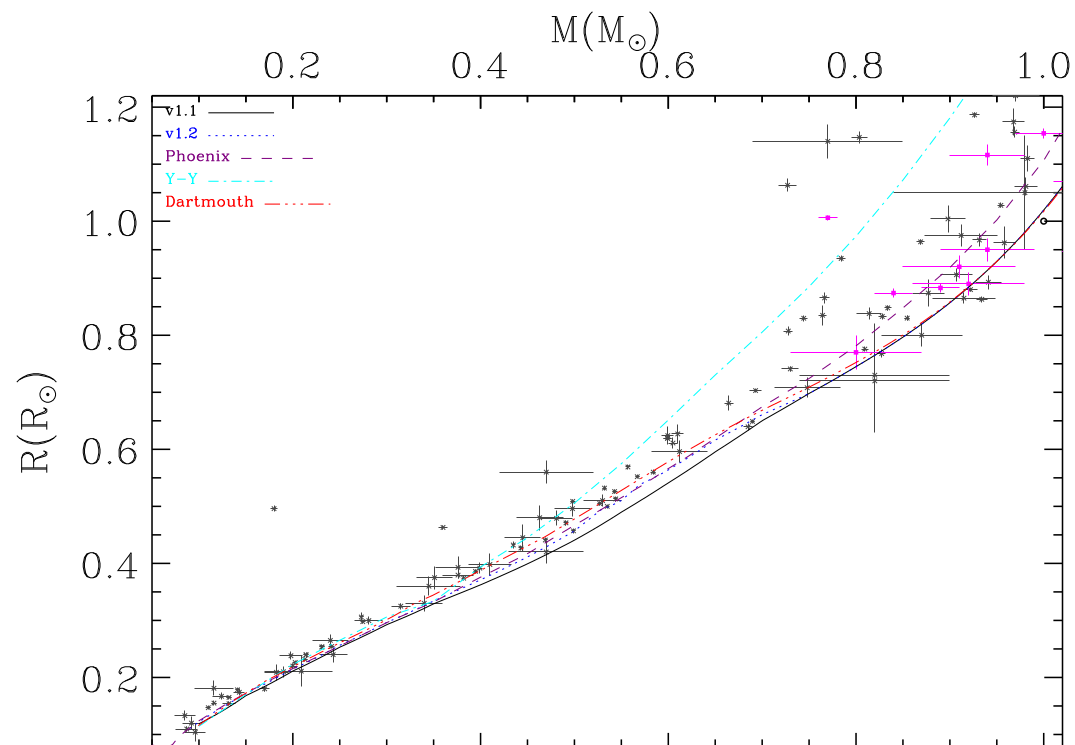
\includegraphics[width=0.8\linewidth]{parsecMRL1}% \\ а)
  \end{minipage}
  \hfill
  \begin{minipage}[ht]{1\linewidth}\centering
    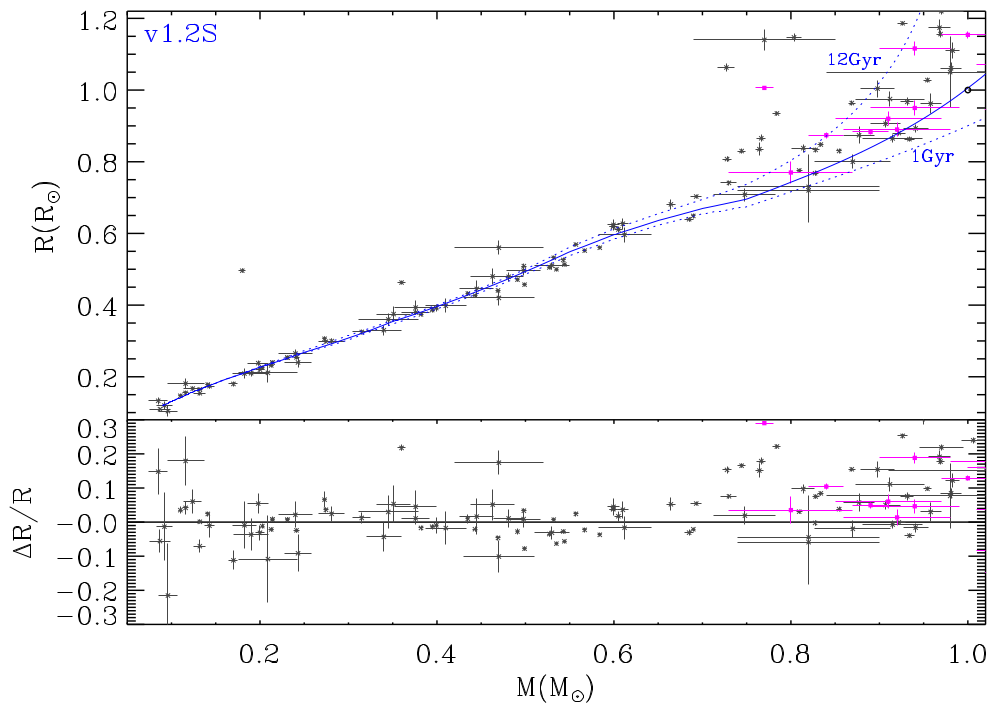
\includegraphics[width=0.8\linewidth]{parsecMRL2}% \\ б)
  \end{minipage}
  \caption{Сверху: эмпирическое отношение <<масса -- радиус>> для звезд с малой массой в солнечной окрестности. Черные звездочки "--- это двойные звезды; пурпурные квадраты "--- одиночные звезды. v1.1 и v1.2 "--- версии изохрон PARSEC (версия 1.2 "--- уточненная при помощи наблюдений нескольких сотен затменно-двойных, для которых есть хорошие кривые лучевых скоростей). Снизу: то же, только построенное для откалиброванного отношения <<T -- $\tau$>> (T "--- температура, $\tau$ "--- средняя оптическая глубина Росселанда) и с добавление изохрон для возрастов 1Gyr и 12Gyr. Взято из \cite{2014MNRAS.444.2525C}, рис. 2 и рис. 12).}
  \label{fig:mrr}
\end{figure}

\begin{figure}[pt]
  \centering
  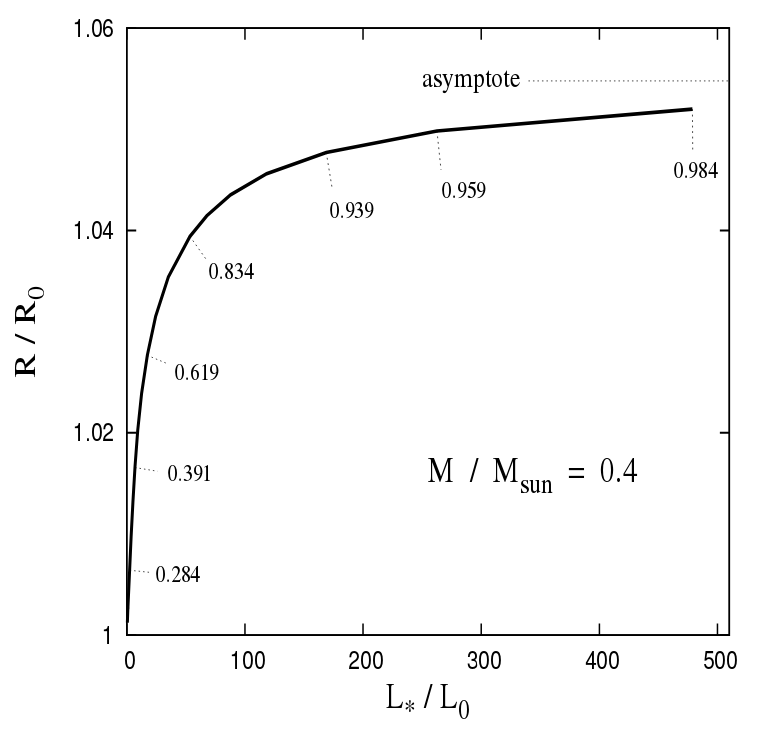
\includegraphics [scale=0.55] {radiusInflationLMSbinary}
  \caption{Попытка оценить влияние <<точечной>> компоненты затменно-двойной (a = 3 \(\textup{R}_0\)) со светимостью \(\textup{L}_*\) (отсечками на кривой показаны значения болометрического альбедо). Взято из \cite{2017A&A...601A..75L}, рис. 4.}
  \label{fig:inf}
\end{figure}

В качестве примера попытки построения эмпирической зависимости <<масса -- светимость>> (MLR) можно отметить работу \cite{2018MNRAS.479.5491E}, где использовались наблюдения звезд с наиболее надежными массами и светимостями. Всего в работу вошло 55 маломассивных объектов. На рисунке~\ref{fig:mlr} представлено сравнение этой модели с аналогичными кривыми по данным MIST и PARSEC, и как можно заметить, модели начинают расходиться при светимости меньше $0.1L_{\odot}$, а  объекты, наблюдаемые в пулковской программе изучения визуально-двойных звезд \cite{2018RAA....18...94S}, лежат у границ погрешностей эмпирической зависимости из работы \cite{2018MNRAS.479.5491E}, обозначенных пунктирной линией. Это тоже указывает на наличие дефицита надежных масс для звезд   M < 0.7~\(\textup{M}_\odot\). Поэтому калибровка существующих моделей карликовых звезд привязана к тесным системам, где оценки M и L могут быть искажены упомянутыми выше систематическими эффектами (несферичность, взаимный нагрев).

\begin{figure}[pt]
  \centering
  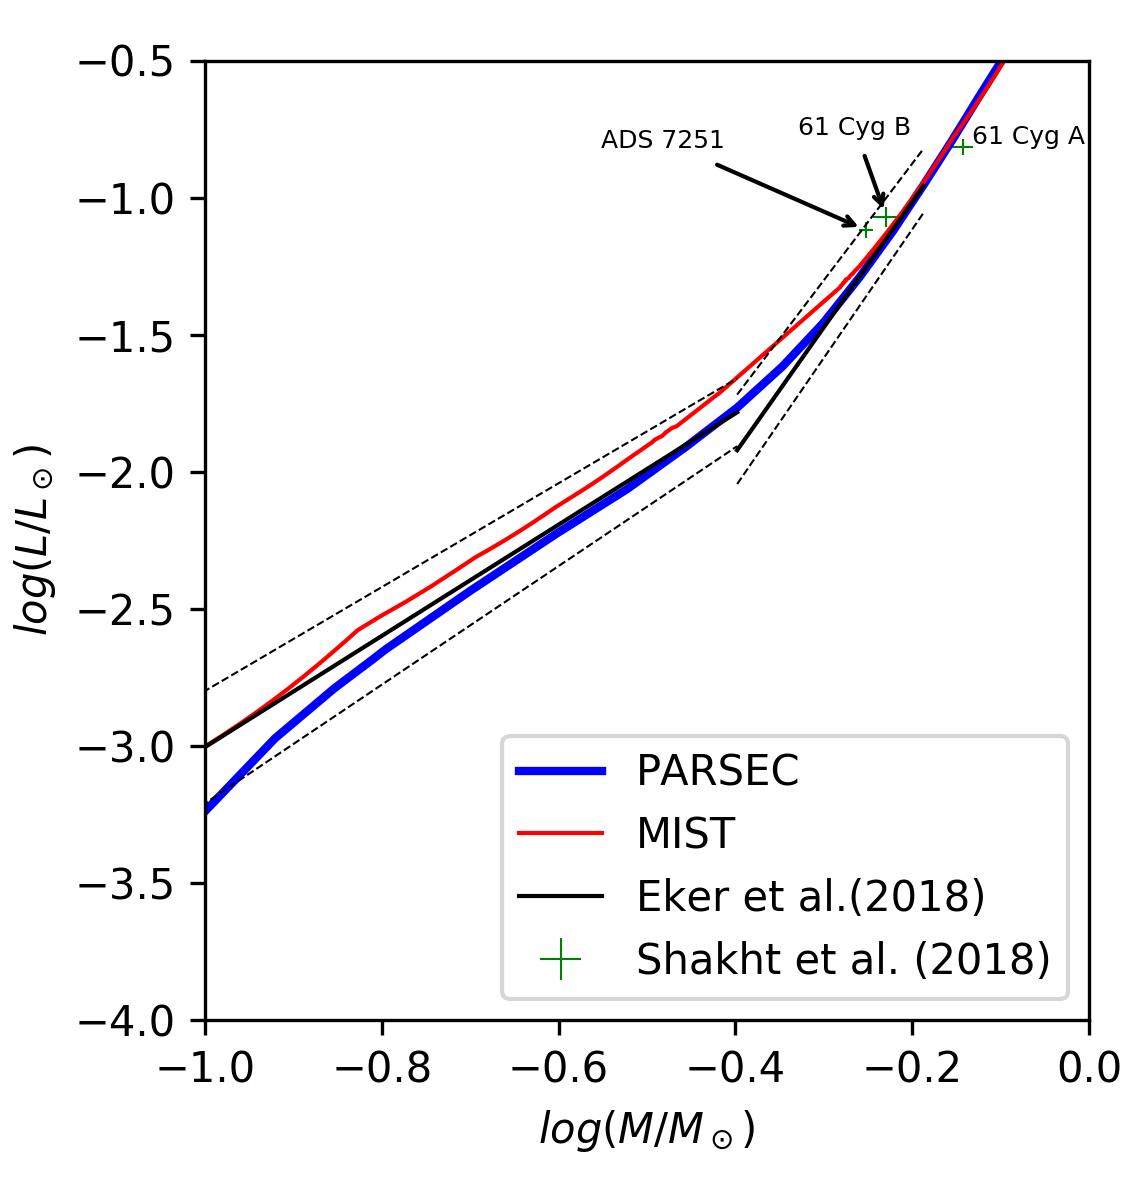
\includegraphics [scale=1.5] {mass-lum}
  \caption{Эмпирическая модель MLR \cite{2018MNRAS.479.5491E} (пунктиром обозначена граница ошибок модели), а также  аналогичные модели проектов PARSEC и MIST. Крестами обозначены визуально-двойные звезды из пулковской программы \cite{2018RAA....18...94S}.}
  \label{fig:mlr}
\end{figure}

\ifsynopsis
\else
Затронутая выше проблема учета конвекционных процессов в маломассивных звездах отмечается и в других работах. Например, в <<Обзоре маломассивных звезд и коричневых карликов>> \cite{2005astro.ph..9798C} говорится о сложности фотометрии звезд класса M5 и более поздних как раз из-за образования на поверхности большого числа звездных пятен и роста видимой активности диска и короны. Авторы объясняют это тем, что конвекция у таких объектов может распространяться вплоть до ядра.  Вообще, в данной работе говорится о целом наборе проблем, связанных с недостатком информации о карликах при их моделировании. На рисунке~\ref{fig:MLch} продемонстрировано, насколько хорошо существующие теоретические зависимости <<масса "--- абсолютная звездная величина>> согласуются с наблюдениями в оптическом диапазоне.

\begin{figure}[pt]
  \centering
  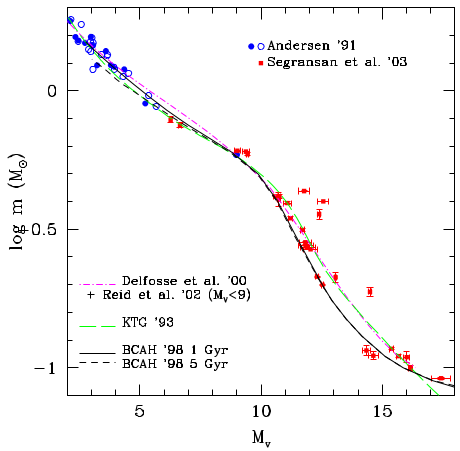
\includegraphics [scale=1.3] {chabrier-et-al-2005-3}
  \caption{Согласие теоретических моделей аналога зависимости <<масса -- звёздная величина>> с наблюдаемыми данными. Заметно расхождение теорий и наблюдений для звезд слабее 10 звездной величины и легче $\approx 0.5$\,\(\textup{M}_\odot\) (этому значению примерно соответствует отсчёт по вертикальной шкале около $-0.3$). Взято из \cite{2005astro.ph..9798C}, рис. 3.}
  \label{fig:MLch}
\end{figure}

Как можно заметить, для звёзд до \(\textup{10}^m\) согласие достаточно хорошее, тогда как более слабые объекты по диаграмме распределены несколько более хаотично и сильнее отклоняются от гладких модельных кривых. В статье говорится, что, вероятно, это связано с образованием большого количество линий поглощения. Исследователи отмечают, что в атмосферах маломассивных звёзд и коричневых карликов образуется множество молекул, чьи конденсаты и частицы сильно влияют на тепловую непрозрачность этих атмосфер. Излучение молекул часто или поглощается в оптическом диапазоне, или слишком слабо из-за эффекта обратного нагрева верхних слоев, где линии формируются. Всё это приводит к видимому покраснению звёзд, в частности, коричневые карлики излучают до 90\,\% своей энергии в ИК полосах, и авторы называют наиболее перспективными исследования данных объектов именно в этом диапазоне. Что согласуется с выводами авторов работы <<Необходимость инфракрасной астрометрии коричневых карликов в эпоху после Gaia>> \cite{2019BAAS...51c.105K}, которые указали на сложности наблюдений Gaia таких объектов. Исследователи отмечают, что диапазон наблюдений Gaia: $\lambda$ < 1,05 мкм \cite{2016A&A...595A...1G}, поэтому подавляющее большинство коричневых карликов, чьи спектры достигают максимума в ИК, не могут быть обнаружены. Например, в ближайших 20 парсеках Gaia может полностью исследовать только типы до L5 \cite{2019ApJS..240...19K}. И в материалах доклада проиллюстрирована необходимость астрометрического мониторинга на более длинных инфракрасных волнах.

Проблема надежного определения радиусов звёзд также упоминается в работе Шабрие \cite{2005astro.ph..9798C}. Отмечается, что используемые сейчас методы определения радиусов могут давать результаты, сильно отличающиеся друг от друга. Значения радиусов, определяемые через оценку наклона кривой блеска у затменных двойных получаются в среднем в 2 раза больше аналогичных радиусов, определенных высокоточной интерферометрией или через эффект гравитационного линзирования. Как уже отмечалось выше, это может быть связано с эффектом взаимного нагрева компонент слишком тесных систем.

Имеет смысл упомянуть об исследованиях по построению и интерпретации функции масс в окрестностях границы <<звёзды -- коричневые карлики>> \cite{2015ApJ...800...72T}. Здесь серьезное внимание уделяется проблеме адекватной оценки доли двойных систем для объектов малых масс. Функция масс претерпевает значимые изменения при разных значениях этой величины.  Это делает весьма актуальной задачу построения полной выборки двойных и кратных звезд в области малых масс. Наша работа имеет целью достичь продвижения в данном направлении.
\fi

Резюмируя вышеизложенное, естественно сделать вывод об актуальности исследования различных типов двойных и кратных систем карликовых звезд, в том числе "--- более широких, порядок периодов которых с одной стороны позволяет строить взаимные орбиты по высокоточным длительным наблюдениям, а с другой стороны "--- пространственное разделение компонент позволяло бы рассматривать каждую из компонент как одиночную звезду, без значительного влияния компаньона (большие полуоси у таких систем составляют порядка 10 а.е.). В современной научной печати можно найти многочисленные примеры работ, посвященных поиску двойных систем, разделению компонент и построению орбит двойных систем  (см., например, \cite{2015csss...18..805C}, \cite{2016ApJ...819...17O}).  

Построение численных моделей процесса звездообразования и дальнейшей динамической эволюции звездной популяции из молекулярных облаков позволяет получить модельные распределения доли двойных систем в зависимости от массы, отношения масс компонент и металличности, проанализировать различные распределения по орбитальным параметрам. Сопоставление результатов таких вычислений с наблюдениями затруднено неполнотой выборки для двойных систем, содержащих маломассивные компоненты. Это является еще одним обоснованием актуальности любых наблюдательных работ, направленных на поиск и изучение двойных и кратных систем среди карликовых звезд.

Сейчас можно найти немало исследований, посвященных построению численных сценариев звездообразования. Например, в работе \cite{2019MNRAS.484.2341B} представлен пример симуляции процесса формирования звездного скопления. Здесь учитывается масса факторов и явлений: химический состав межзвездной среды, влияние космических лучей, нагрев газа и пыли из-за излучения звезд, процессы диффузии и переноса излучения. В итоге модельное облако M = 500 \(\textup{M}_\odot\) порождает порядка сотни звезд суммарной массы $\approx$\,100~\(\textup{M}_\odot\) с медианной массой 0,15 \(\textup{M}_\odot\). Как видно из рисунка~\ref{fig:imf}, получившаяся функция масс наилучшим образом согласуется с результатами построения IMF (Initial Mass Function "--- начальная функция масс) \cite{2005ASSL..327...41C}, собравшим наблюдения маломассивных звезд и коричневых карликов на протяжении 50 лет.  Особое место в исследовании отведено изучению доли и свойств кратных объектов. Как следует из рисунка~\ref{fig:fract}, доля кратных систем в получившейся модели растёт с увеличением начальных масс объектов, и этот результат подтверждают и эмпирические данные. Причем исследователи отмечают, что так как доля кратных систем имеет явную корреляцию с значениями начальных масс, то при сравнении моделирования с наблюдениями всегда стоит использовать аналогичные диапазоны масс. На рисунке~\ref{fig:hist} представлено сравнение получившейся гистограммы распределения двойных, тройных и четверных систем по большим полуосям (тройные системы дают два значения полуосей, а четверные "--- три) с двумя эмпирическими построениями: для M-карликов и звезд с начальными массами солнечного типа. Отмечается, что поскольку большинство моделируемых объектов имеют малую массу, то ожидается, что распределение для M-карликов должно лучше соответствовать модели, и этот результат в большей мере воспроизводит гистограмма для двойных систем.  Попытка воссоздания эволюции доли двойных систем для звездных скоплений с различными начальными параметрами представлена, например, в работе \cite{2007ApJ...665..707H}. На рисунке~\ref{fig:evol} представлен результат моделирования эволюции доли двойных систем в кластере из 100~000 звезд, где в начальный заданный момент времени доля двойных составляла 10\,\%. Из рисунка видно, что с течением времени прогнозируемое моделью число кратных систем имеет явный тренд к возрастанию.

\begin{figure}[pt]
  \centering
  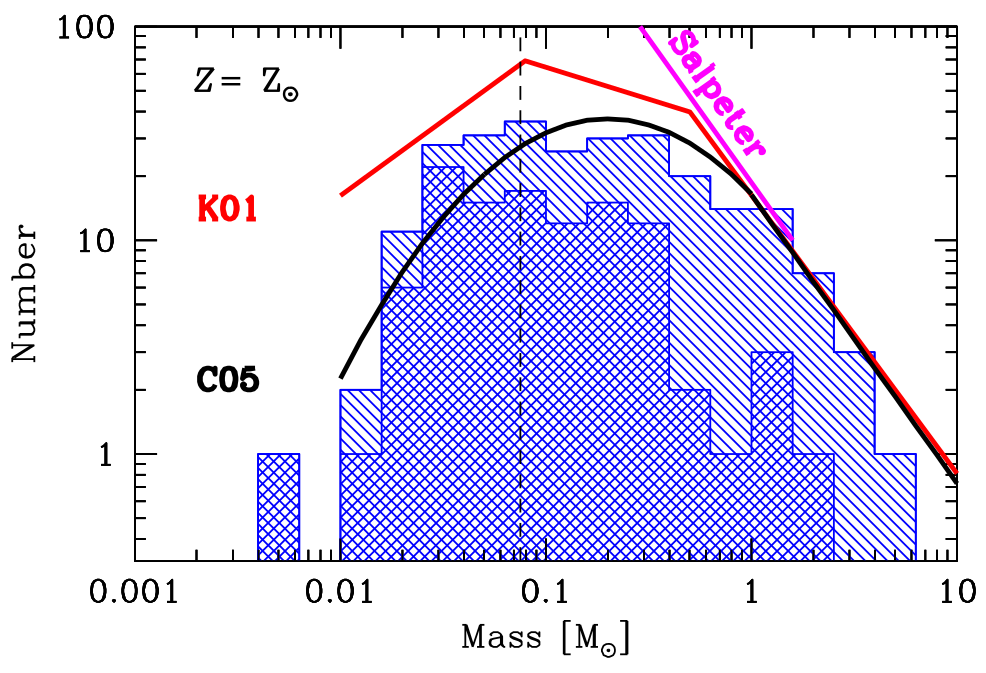
\includegraphics [scale=0.45] {Bate-IMF}
  \caption{IMF для звезд и коричневых карликов солнечной металличности в рамках численной модели \cite{2019MNRAS.484.2341B}. Двойная штриховка "--- объекты без аккреции, одиночная штриховка "--- с аккрецией. Функции масс хорошо согласуются с данными \cite{2005ASSL..327...41C} (С05). Также представлены две другие IMF: Salpeter~\cite{1955ApJ...121..161S} и K01~\cite{2001MNRAS.322..231K}. Взято из \cite{2019MNRAS.484.2341B}, рис. 8, нижний левый.}
  \label{fig:imf}
\end{figure}

\begin{figure}[pt]
  \centering
  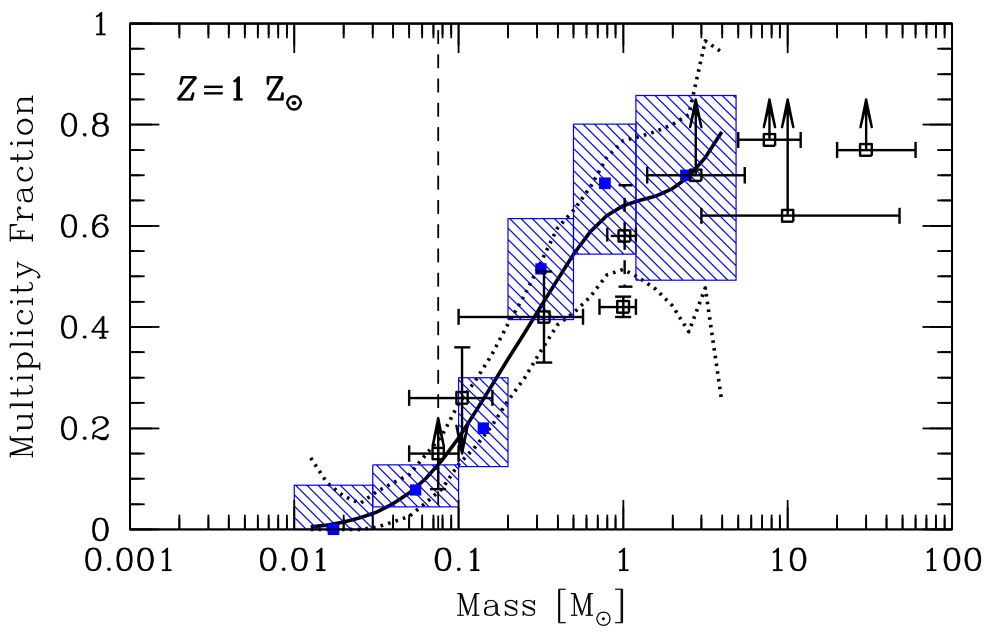
\includegraphics [scale=0.47] {Bate-BF}
  \caption{Доля кратности в зависимости от первичной массы звезд солнечной металличности в рамках численной модели \cite{2019MNRAS.484.2341B}. Синие закрашенные квадраты, окруженные заштрихованными областями, представляют результаты численных расчетов со статистической погрешностью 1$\sigma$. Толстая сплошная линия "--- кривая долей кратности, вычисленная с использованием скользящего логарифма, пунктирные линии "--- на 1$\sigma$-интервале вокруг нее. Незакрашенные квадраты с погрешностями и пределами "--- наблюдаемые доли кратных из исследований \cite{2003ApJ...587..407C}, \cite{2006AJ....132..663B}, \cite{1992ApJ...396..178F}, \cite{2010ApJS..190....1R}, \cite{1991A&A...248..485D}, \cite{2007A&A...474...77K}, \cite{2013MNRAS.436.1694R}, \cite{1999NewA....4..531P} и \cite{1998AJ....115..821M} слева направо.  Исследователи отмечают, что наблюдаемая тенденция увеличения кратности воспроизводится всеми рассмотренными расчетами, и поскольку доля кратных сильно зависит от начальных масс, важно, чтобы при сравнении моделей с наблюдениями использовались аналогичные массы. Взято из \cite{2019MNRAS.484.2341B}, рис. 10, нижний левый.}
  \label{fig:fract}
\end{figure}

\begin{figure}[pt]
  \centering
  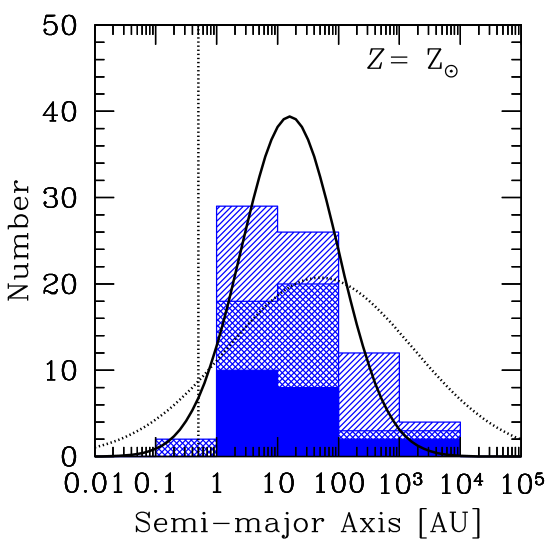
\includegraphics [scale=0.8] {Bate-a-distr}
  \caption{Гистограмма распределения кратных звезд солнечной металличности с начальными массами > 0.1Msun по большим полуосям в рамках численной модели \cite{2019MNRAS.484.2341B}.  Бары с одиночной, двойной и сплошной штриховкой представляют двойные, тройные и четверные системы соответственно. Сплошная кривая "--- распределение M-карликов из обзора \cite{2012ApJ...754...44J}, а пунктирная "--- распределение звезд с начальными массами солнечного типа из обзора \cite{2010ApJS..190....1R}. Поскольку большинство моделируемых систем имеют малую массу, ожидается, что распределение \cite{2012ApJ...754...44J} будет соответствовать лучше, чем \cite{2010ApJS..190....1R}. Вертикальная пунктирная линия показывает предел разрешающей способности расчетов, который определяется радиусами аккреции поглощающих частиц (0,5 а.е.). Взято из \cite{2019MNRAS.484.2341B}, рис. 11, третий слева.}
  \label{fig:hist}
\end{figure}


\begin{figure}[pt]
  \centering
  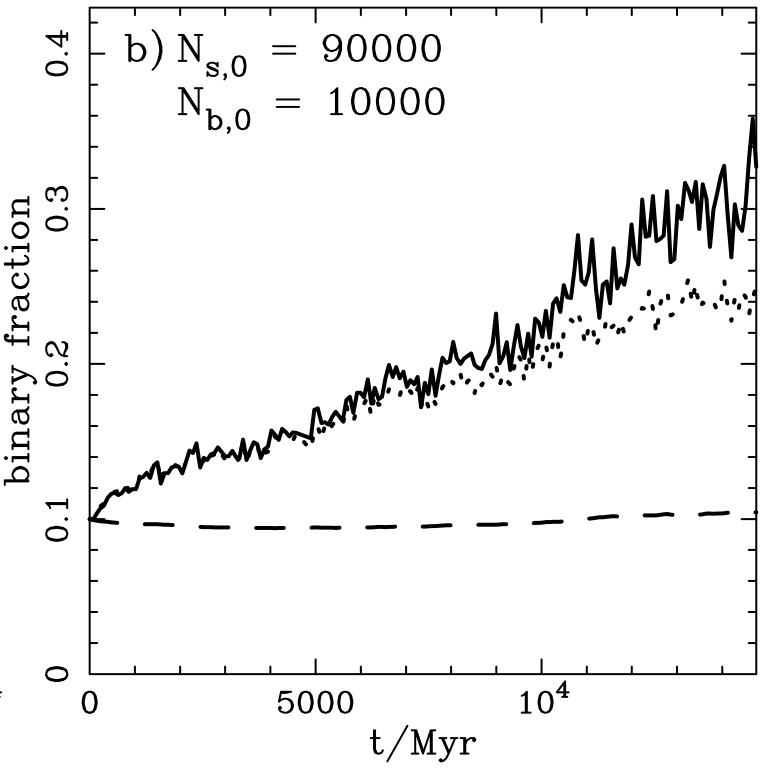
\includegraphics [scale=0.5] {Hurley}
  \caption{Эволюция доли двойных систем в ядре (сплошная линия), в пределах 10\,\% радиуса Лагранжа (пунктирная линия) и для всего кластера (пунктирная линия) в одной из моделей. $N_{s,0}$, $N_{b,0}$ "---  количества одинарных и двойных звезд соответственно в исходной модели.  Взято из \cite{2007ApJ...665..707H}, рис. 7b.}
  \label{fig:evol}
\end{figure}

Однако, пока сложно утверждать, что даже совокупность существующих обзоров и программ решает проблему в полной мере. К сожалению, несмотря на существенный прогресс в исследовании кратных систем, который дает Gaia DR2, даже после значительного исправления первого релиза, данные миссии также не дают полноты выборки для визуальных двойных звезд с разделением $\rho$ менее $2''$ (рисунок~\ref{fig:compl}), что отмечают и авторы \cite{2018A&A...616A..17A},\cite{2018A&A...616A...2L}. Это может быть связано со сложностью анализа изображения тесных систем в Gaia DR2 \cite{2016A&A...595A...3F}, когда FWHM (ширина на полувысоте) становится меньше углового разделения $\rho$ (см. рисунок~\ref{fig:spf}). Сложность разделения тесных систем сказывается и на ошибках определения пиксельных координат, что в свою очередь влияет на вычисляемые значения собственных движений и параллаксов. Например, на рисунке~\ref{fig:err} можно увидеть, как относительная точность параллаксов Gaia DR2 падает при $\rho$~<~$2''$. Кроме того, отмечается проблема кросс-идентификации быстрых объектов ($\mu$~>~100 mas/yr), которые в основном как раз относятся к ближайшему звездному населению. Как указано в GaiaDR2 Documentation 1.2\footnote{\textit{https://gea.esac.esa.int/archive/documentation/GDR2/index.html}}, для звезд с разделением менее $0.7''$ всегда будет стоять проблема кросс-идентификации, и поэтому объекты Gaia DR2 с флагом <<duplicate source>> предлагается отдельно проверять, являются ли они действительно дубликатами одиночной звезды или же входят в двойную или кратную систему. Помимо проблемы отождествления тесных объектов, стоит упомянуть, что период наблюдений миссии Gaia строго ограничен и не дает возможности получения достаточного количества наблюдений для построения орбит широких пар, периоды взаимного обращения которых сильно превалируют над сроком жизни космического аппарата.

\begin{figure}[pt]
  \centering
  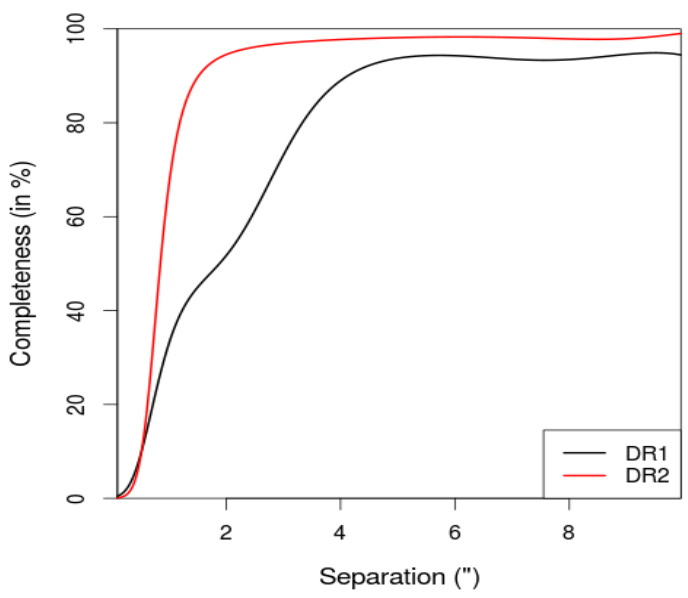
\includegraphics [scale=0.6] {gaia-complitness-for-binaries}
  \caption{Полнота (\%) визуальных двойных звёзд из каталога WDS в зависимости от разделения между компонентами (WDS), детектируемых в ходе миссии Gaia.  Gaia DR1 (черный), Gaia DR2 (красный). Заметно снижение полноты выборки двойных для тесных систем ($\rho$ < 2 arcsec). Взято из \cite{2018A&A...616A..17A}, рис. 8.}
  \label{fig:compl}
\end{figure}

\begin{figure}[pt]
  \centering
  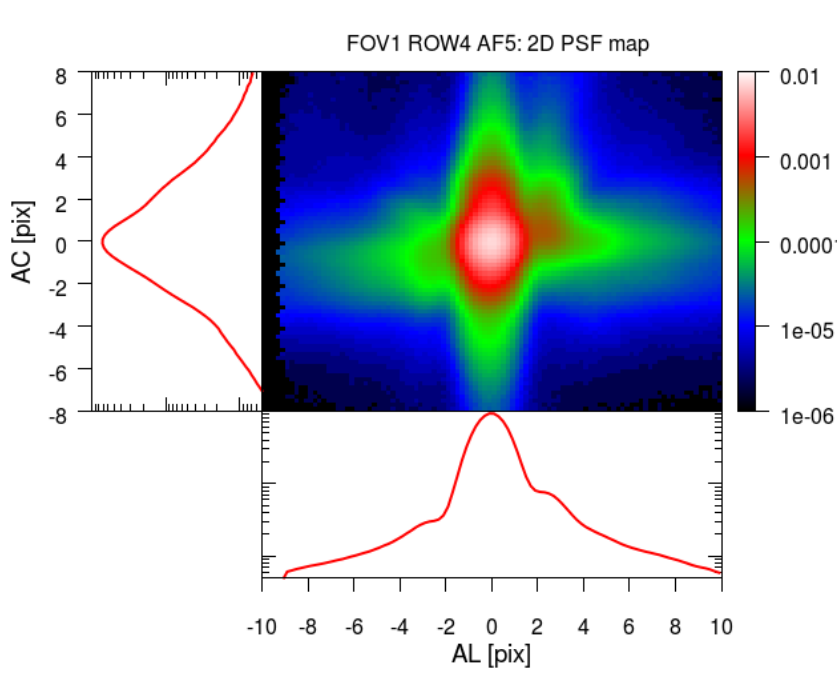
\includegraphics [scale=0.6] {gaia-psf}
  \caption{PSF изображения тесной двойной (1.2$''$ на 2.8$''$) демонстрирует сложность разделения в Gaia DR2 изображений подобных звезд. Взято из \cite{2016A&A...595A...3F},  рис. 7.}
  \label{fig:spf}
\end{figure}

\begin{figure}[pt]
  \centering
  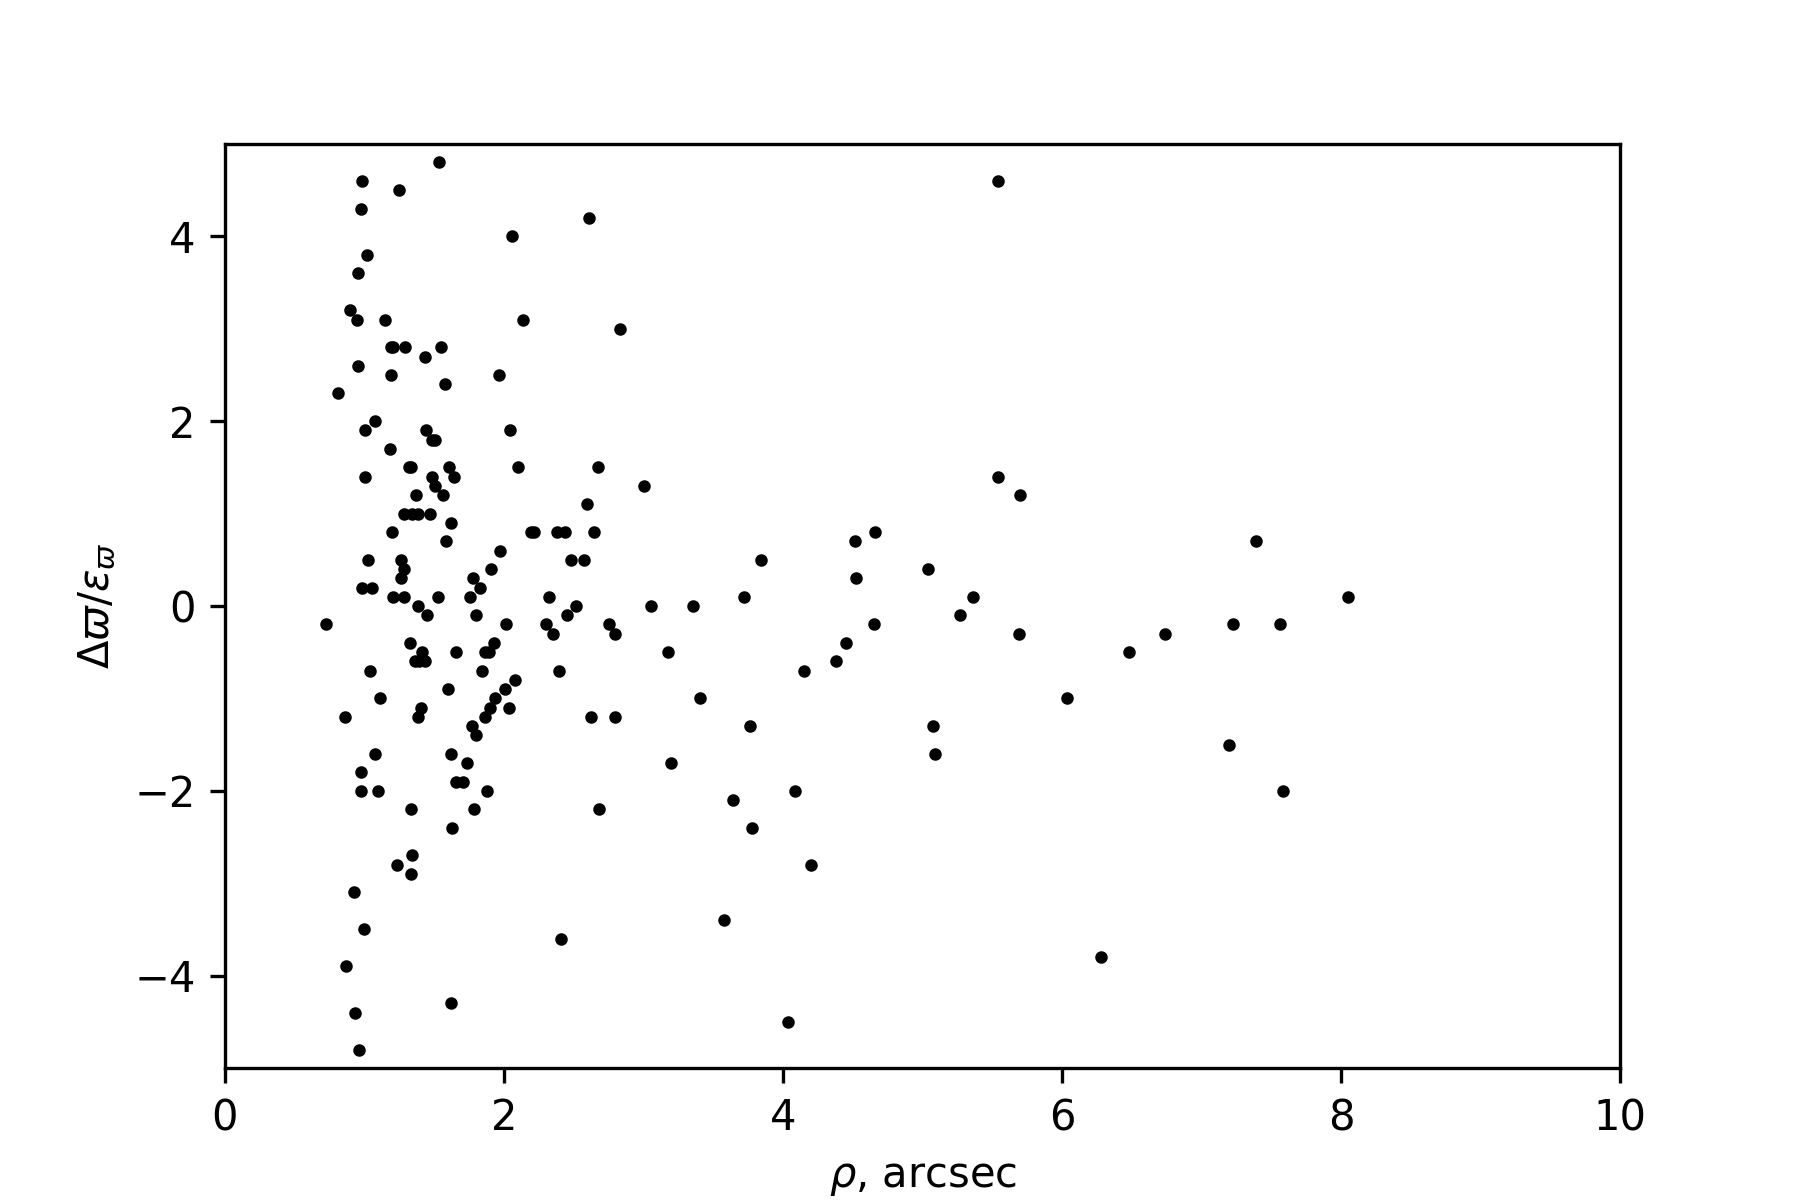
\includegraphics [scale=1.2] {delta_pi-vs-rho}
  \caption{Увеличение разброса относительных ошибок параллаксов Gaia для изображений звезд с разделением менее 3$''$ указывает на существенное снижение точности определения пиксельных координат компонент.}
  \label{fig:err}
\end{figure}

В связи с указанными проблемами важным становится применение всех доступных методик детектирования кратности звезд и использование по возможности всех доступных наблюдений звезд, охватывающих широкий диапазон эпох. Исследования звезд в ближайших 50 пк от Солнца дают возможность наиболее эффективного их применения. Как можно убедиться из рисунка~\ref{fig:sepdis}, для звездных систем с величинами больших полуосей порядка 10 а.е. видимое разделение компонент даже в ближайшем окружении составляет меньше $1''$. К счастью, существующие методы высокого разрешения (спекл-интерферометрия, метод удачных экспозиций) позволяют разделять объекты $\rho$~<~$1''$ (см. рисунок~\ref{fig:lucky}). Однако данные методы сложно применять массово, так как требуют таргетированных и часто многочисленных наблюдений, и больше подходят для построения орбит уже выявленных двойных и кратных систем.

\begin{figure}[pt]
  \centering
  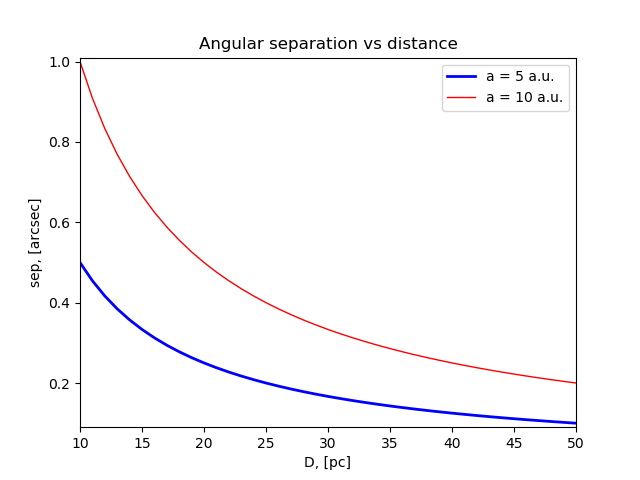
\includegraphics [scale=1.1] {separation-vs-distance}
  \caption{Зависимость видимого углового разделения компонент систем с заданными большими полуосями от гелиоцентрического расстояния. Поиск и определение динамических параметров маломассивных двойных систем "--- актуальная задача, требующая наблюдений широкого класса объектов, для которых разделение $\rho$~<~FWHM.}
  \label{fig:sepdis}
\end{figure}

\begin{figure}[pt]
  \centering
  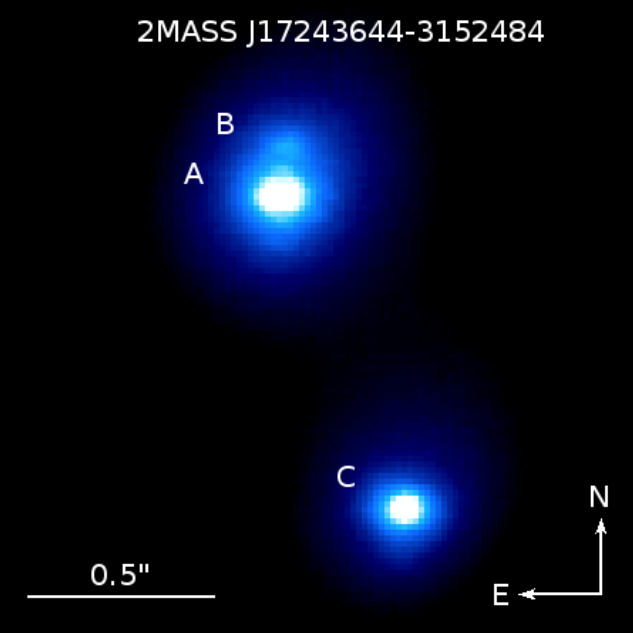
\includegraphics [scale=0.6] {lucky-imaging-example}
  \caption{Рис 15. 3.5m New Technology Telescope (NTT) "--- метод удачных экспозиций (Lucky imaging). Взято из \cite{2017A&A...599A..70J}, рис. 1. }
  \label{fig:lucky}
\end{figure}

Близость исследуемых объектов позволяют эффективно применять различные методы современной астрономии для их изучения. Например, наиболее заметные смещения компонент близких систем по лучу зрения дают возможность плодотворно выявлять оптически неразрешаемые спектрально-двойные звезды благодаря значительному проявлению эффекта доплеровского смещения спектральных линий. Однако, объектами таких исследований становятся в основном всё те же тесные системы, массы и радиусы которых сложно использовать для построения моделей одиночных звезд.

Целью данной работы является разработка метода поиска двойных и кратных звезд, дальнейшее определение орбитальных параметров которых позволят получить более надежные массы, радиусы и светимости маломассивных звезд и коричневых карликов и уточнить фундаментальные закономерности для этих групп объектов. Исследуемые системы преимущественно должны быть не слишком тесными, чтобы компоненты не влияли в значительной мере на характеристики друг друга, а их периоды составляли несколько десятилетий, что дает возможность построить орбиту по короткой дуге за относительно небольшой отрезок времени. Поэтому объектами наших поисков являются двойные звезды низкой светимости из ближайшего окружения Солнца, большие полуоси взаимных орбит которых составляют примерно 5--10 а.е.. Как уже отмечалось, даже в ближайшей солнечной окрестности такие системы часто разрешимы только  с помощью наблюдений методами высокого разрешения  (спекл-интерферометрия, метод удачных экспозиций), которые пока не удается использовать для массовых наблюдений. Поэтому одна из задач данного исследования состоит в разработке методов обнаружения искомых двойных систем, основанных на подходах традиционной наземной оптической астрометрии и анализа изображений.

Актуальность рассматриваемых проблем способствовала тому, что в XX в. было реализовано несколько проектов, направленных на обнаружение быстрых звезд \cite{1955AJ.....60..274D}, \cite{1979nlcs.book.....L} и на определение их собственных движений и тригонометрических параллаксов \cite{1995gcts.book.....V}. Научные группы из различных обсерваторий прилагают усилия в этом направлении. Большой цикл работ по данной тематике представляет команда проекта RECONS (см., например, \cite{2017AJ....153...14W}), имеются существенные результаты в рамках проекта MEarth \cite{2017ApJ...836..124D}. Часть исследований в рамках пулковской программы по изучению звезд с большими собственными движениями имела целью детектирование двойных систем, о чем свидетельствует цикл работ: \cite{2011AstL...37..420K}, \cite{2015AstL...41..833K}, \cite{2016AstL...42..686K}.

\newpage

Подводя итог вводной части работы коротко резюмируем основные моменты.
% {\progress}
% Этот раздел должен быть отдельным структурным элементом по
% ГОСТ, но он, как правило, включается в описание актуальности
% темы. Нужен он отдельным структурынм элемементом или нет ---
% смотрите другие диссертации вашего совета, скорее всего не нужен.

{\aim} данной работы является выявление двойных систем среди близких к Солнцу маломассивных карликовых звезд. 

Для~достижения поставленной цели необходимо было решить следующие {\tasks}:
\begin{enumerate}
  \item оценить полноту современных обзоров и списков двойных систем;
  \item сформировать список звезд для исследования;
  \item разработать методы быстрого и массового поиска двойных систем среди близких к Солнцу маломассивных карликов, основанные на подходах наземной оптической астрометрии и анализа цифровых изображений звездообразных объектов.
\end{enumerate}

Актуальность данного исследования обусловлена недостатком надежных оценок масс для карликовых звезд, затрудняющим построение их физических моделей с одной стороны, и необходимостью верификации численных моделей формирования звездных популяций, в которой важную роль играют эмпирические распределения двойных систем по ряду параметров, с другой стороны.

{\novelty}
\begin{enumerate}
  \item Были предложены новые варианты методик поиска двойных систем на основе анализа собственных движений и путем анализа формы изображений звезд на ПЗС-кадрах;
  \item Выполнены собственные ПЗС-наблюдения, позволившие произвести проверку адекватности разработанных методов и выявить 259 звезд-кандидатов в двойные системы;
  \item В результате спекл-интерферометрических наблюдений на БТА САО РАН и 2.5 м телескопе КГО ГАИШ МГУ впервые детектирована двойственность систем J1158+4239, J1135+0414, J1147+6050, независимо подтверждены ранее уже выявленные двойные звезды J1601+3714, J0259+3636.
\end{enumerate}

Теоретическая значимость работы определяется модификацией метода Вилена, позволяющей выявлять двойственность звезд путем анализа собственных движений на основе ПЗС-кадров и сканов фотопластинок с общей системой опорных звезд; адаптацией шейплет-формализма для оценивания эллиптичности и асимметрии звездных изображений на ПЗС-кадрах.

{\influence} состоит в проведении большого цикла астрономических наблюдений на Нормальном астрографе и метровом телескопе «Сатурн» в Пулковской обсерватории, анализ результатов которого позволил выявить двойственность упомянутых выше звезд. Важно, что представленные методы реализованы в виде программного обеспечения, которое может быть адаптировано для других инструментов различных обсерваторий.

{\methods} За основу исследований были взяты зарекомендовавшие себя технологии исследования быстрых звезд ($\Delta\mu$-двойные) и анализа изображений (shapelet-декомпозиция), которые были адаптированы с учетом исследуемого материала и успешно применены для поиска двойных звезд среди близких карликов.

{\defpositions}
\begin{enumerate}
  \item Модификация метода Вилена по выявлению звезд-кандидатов в $\Delta\mu$-двойные;
  \item Адаптация шейплет-формализма для детектирования скрытых двойных звездных изображений;
  \item Выявление 259 звезд--кандидатов в маломассивные двойные системы;
  \item Подтверждение двойственности пяти систем методами высокого разрешения.
\end{enumerate}


{\reliability} полученных результатов обеспечивается частичным присутствием найденных двойных звезд в существующих каталогах двойных звезд, в том числе "--- WDS, подтверждением двойственности звезд на спекл-изображениях.


{\probation}
Детальное изложение методов и результатов работы представлено в четырех публикациях, индексируемых в наукометрических базах данных (web of science, Scopus и т.п.), в устных докладах на российских и международных конференциях (астрометрические конференции <<Пулково--2012>>, <<Пулково--2015>>, <<Пулково--2018>>; ВАК--2013 (Санкт-Петербург); ВАК--2016 (Нижний Архыз); <<Современная астрометрия>> (Москва)), астрометрических семинарах Пулковской обсерватории и Пулковских молодежных конференциях. Кроме того, результаты исследований доступны в астрономических базах данных (CDS, WDS).
%\textbf{Публикации.} Основные результаты по теме диссертации изложены в 4 печатных изданиях. Из них 3 изданы в журналах, рекомендованных ВАК, 4 индексируются в Scopus (1 работа является материалами конференции), 3 индексируются в Web of Science. 

{\contribution} Автор принимал активное участие во многих этапах работы: наблюдения на пулковских  телескопах (Нормальном астрографе и телескопе <<Сатурн>>), написание программного обеспечения для вычисления и анализа собственных движений звезд, написание текстов для совместных с соавторами научных статей, выступления на научных конференциях с устными докладами, посвященными настоящему исследованию. 


%\ifnumequal{\value{bibliosel}}{0}
{%%% Встроенная реализация с загрузкой файла через движок bibtex8. (При желании, внутри можно использовать обычные ссылки, наподобие `\cite{vakbib1,vakbib2}`).
    %{\publications}% Основные результаты по теме диссертации изложены в XX печатных изданиях,
    %X из которых изданы в журналах, рекомендованных ВАК,
    %X "--- в тезисах докладов.
}% 
{%%% Реализация пакетом biblatex через движок biber
    %\begin{refsection}[bl-authorvak,bl-authorwos,bl-authorscopus,bl-authorother,bl-authorconf]
        % Это refsection=1.
        % Процитированные здесь работы:
        %  * подсчитываются, для автоматического составления фразы "Основные результаты ..."
        %  * попадают в авторскую библиографию, при usefootcite==0 и стиле `\insertbiblioauthor` или `\insertbiblioauthorgrouped`
        %  * нумеруются там в зависимости от порядка команд `\printbibliography` в этом разделе. 
        %  * при использовании `\insertbiblioauthorgrouped`, порядок команд `\printbibliography` в нём должен быть тем же (см. biblio/biblatex.tex)
        %
        % Невидимый библиографический список для подсчёта количества публикаций:
        %\printbibliography[heading=nobibheading, section=1, env=countauthorvak,    keyword=biblioauthorvak]%
        %\printbibliography[heading=nobibheading, section=1, env=countauthorwos,    keyword=biblioauthorwos]%
        %\printbibliography[heading=nobibheading, section=1, env=countauthorscopus, keyword=biblioauthorscopus]%
        %\printbibliography[heading=nobibheading, section=1, env=countauthorconf,   keyword=biblioauthorconf]%
        %\printbibliography[heading=nobibheading, section=1, env=countauthorother,  keyword=biblioauthorother]%
        %\printbibliography[heading=nobibheading, section=1, env=countauthor,       keyword=biblioauthor]%
        %
        % Цитирования.
        %  * Порядок перечисления определяет порядок в библиографии (только внутри подраздела, если `\insertbiblioauthorgrouped`).
        %  * Если не соблюдать порядок "как для \printbibliography", нумерация в `\insertbiblioauthor` будет кривой.
        %  * Если цитировать каждый источник отдельной командой --- найти некоторые ошибки будет проще.
        %
        %% authorvak
        %\nocite{vakbib1}%
        %\nocite{vakbib2}%
        %\nocite{vakbib3}
        %
        %% authorwos
        %\nocite{wosbib1}%
        %
        %% authorscopus
        %\nocite{scbib1}%
        %
        %% authorconf
        %\nocite{confbib1}%
        %\nocite{confbib2}%
        %
        %% authorother
        %\nocite{bib1}%
        %\nocite{bib2}%
        %\nocite{bib3}
        %\nocite{bib4}
        %\nocite{bib5}
        %
        %
        %{\publications} Основные результаты по теме диссертации изложены в~\arabic{citeauthor}~печатных изданиях,
        %\newcounter{citeauthorscwostot}% сумма citeauthorscopus и citeauthorwos
        %\setcounter{citeauthorscwostot}{\value{citeauthorscopus}}%
        %\addtocounter{citeauthorscwostot}{\value{citeauthorwos}}%
        %\arabic{citeauthorvak} из которых изданы в журналах, рекомендованных ВАК\sloppy%
        %\ifnum \value{citeauthorscwostot}>0%
        %    , \arabic{citeauthorscwostot} "--- в~периодических научных журналах, индексируемых Web of Science и Scopus\sloppy%
        %\fi%
        %\ifnum \value{citeauthorconf}>0%
        %    , \arabic{citeauthorconf} "--- в~тезисах докладов.
        %\else%
        %    .
        %\fi
    %\end{refsection}%
    %\begin{refsection}[bl-authorvak,bl-authorwos,bl-authorscopus,bl-authorother,bl-authorconf]
        % Это refsection=2.
        % Процитированные здесь работы:
        %  * попадают в авторскую библиографию, при usefootcite==0 и стиле `\insertbiblioauthorimportant`.
        %  * ни на что не влияют в противном случае
        %\nocite{vakbib2}%vak
        %\nocite{bib1}%other
        %\nocite{confbib1}%conf
    %\end{refsection}%
	%
	% Всё, что вне этих двух refsection, это refsection=0,
	%  * для диссертации - это нормальные ссылки, попадающие в обычную библиографию
	%  * для автореферата:
	%     * при usefootcite==0, ссылка корректно сработает только для источника из `external.bib`. Для своих работ --- напечатает "[0]" (и даже Warning не вылезет).
	%     * при usefootcite==1, ссылка сработает нормально. В авторской библиографии будут только процитированные в refsection=0 работы.
}
